%!TEX program = xelatex
% 完整编译: xelatex -> bibtex -> xelatex -> xelatex

\documentclass[lang=cn,10pt,a4paper]{elegantpaper}
\usepackage{listings}
\usepackage{xcolor}
\title{浙江大学休闲餐厅排队制度研究}
\author{冯相 \and 王艺瑾 \and 徐润森 \and 占子越 \and 宗威旭 \\3180102776}
\institute{浙江大学}

\date{\zhtoday}

\begin{document}

\maketitle

\begin{abstract}
本文基于食堂排队取餐这一实际问题,选取排队取餐方案能否相比随即取餐节省取餐时间这一研究问题,通过建立周期模型、概率模型、混乱模型三种不同模型进行探讨,并对于不同模型的效果进行了比较与评估。对于这一实际问题,我们通过建立数学模型的方法进行研究分析,并针对分析结果进行了检验与建议。并给出了我们的思考与收获
\keywords{数学建模,排队问题,排队论}
\end{abstract}

\section{介绍}
\subsection{问题背景}
2019年11月起,浙江大学紫金港校区的休闲餐厅将取餐方式由原先的自由取餐变为排队按顺序经过取餐台取餐并结账的方式(如图1)。这一取餐制度的转变引起了学校同学们的热议。有人认为取餐时间变短了,有人认为取餐时间变长了。针对休闲餐厅这一排队制度,我们将其抽象出来,并使用数学模型进行描述,尝试从中得到取餐时间的数学表达式,并对食堂提高同学们取餐效率提出合理的建议。\\
\begin{figure}[htbp]
  \centering
  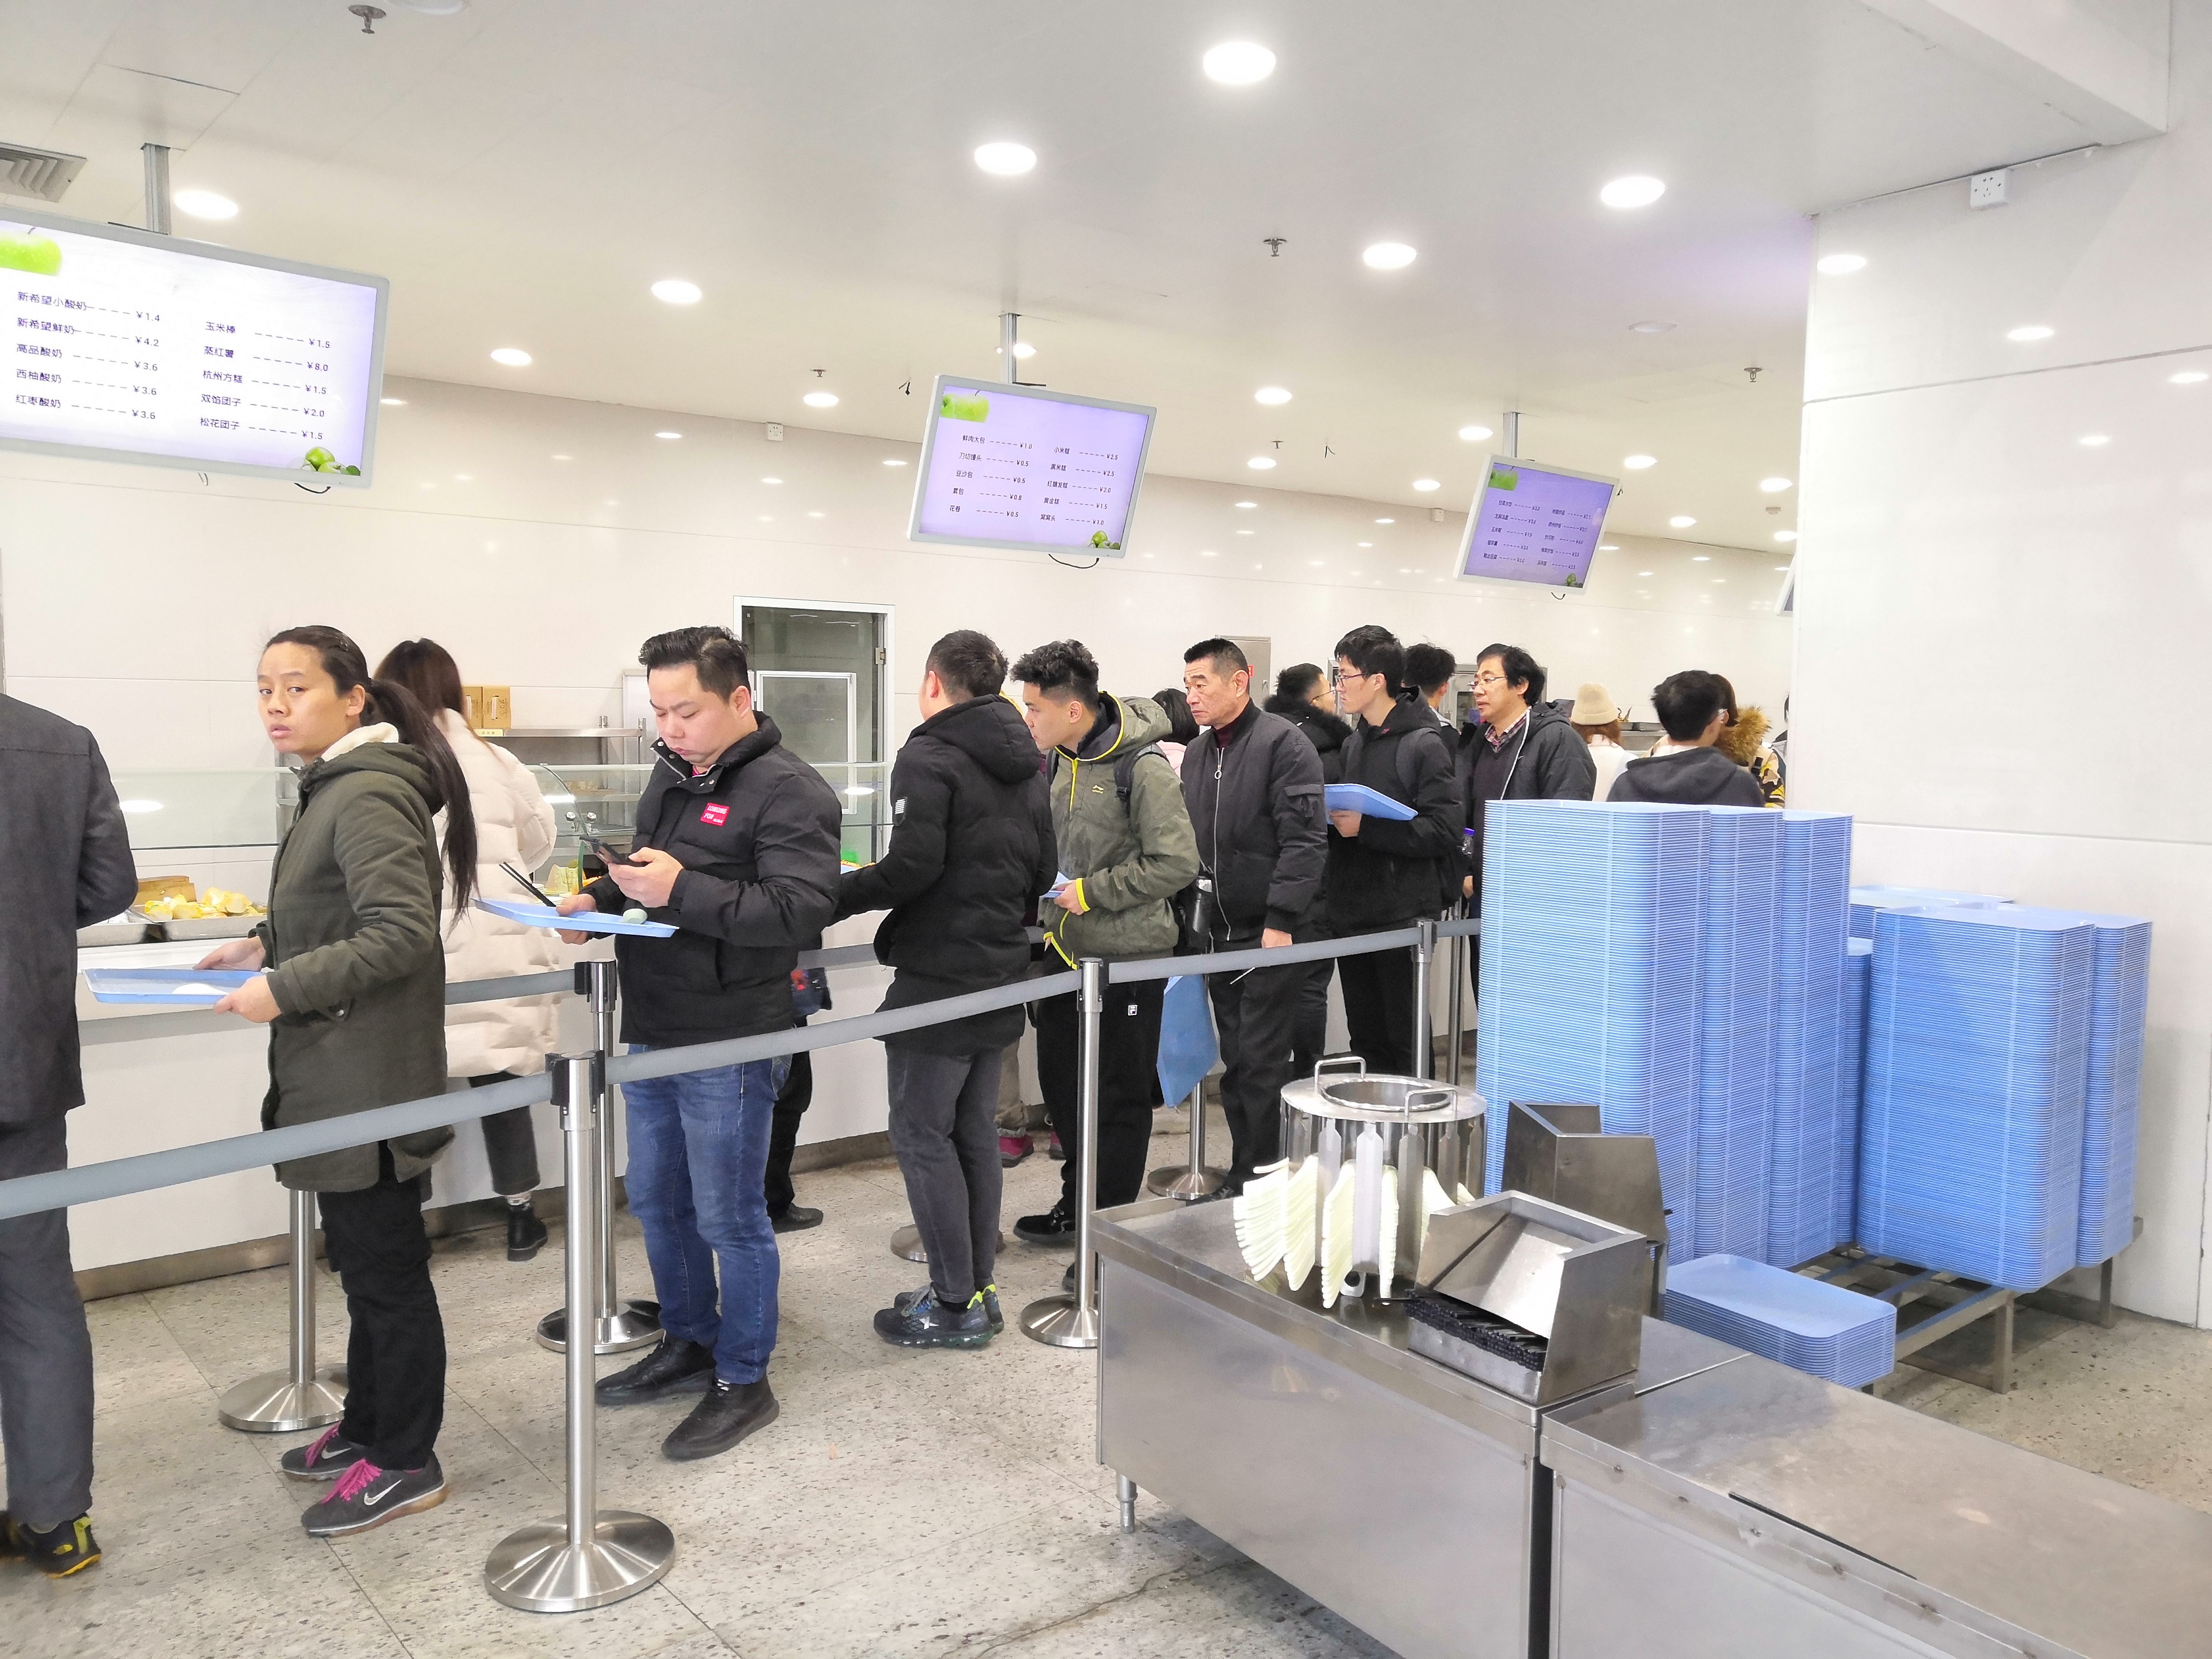
\includegraphics[scale=0.07]{./image/pic1.jpg}
  \caption{休闲食堂排队取餐}
\end{figure}
\section{建模}
\subsection{周期模型}
在非用餐高峰期,我们认为一个人取菜的过程是畅通无阻的。因此,我们将目光集中在探究高峰时期人员取菜的情况。为了简化情况,突出问题的本质,我们作出以下假设:
\begin{itemize}
\item 人流是连续不断的,即除一个人取菜时,后面的人会立刻跟上前面的移动
\item 每个人在取菜过程中会且只会取一个菜,设每个人取任何一道菜的时间都为$\Delta t$
\item 所有的菜在同学中的受欢迎程度是相同的,且菜的种类共有$S$种,恰好与所有取菜台前可以站立的同学人数之和相等,即在取菜走廊的$S$个位置均有菜可以取
$N_{sum}$ 为在食堂用餐的总人数,$T_{0}$ 为一个人在畅通无阻的情况下走过全路程而不取菜的时间。
\end{itemize}


同时,​我们设置以下常量使问题描述简化:$N_{sum}$ 为在食堂用餐的总人数,$T_{0}$ 为一个人在畅通无阻的情况下走过全路程而不取菜的时间。此外,我们称因为某一个人在取菜而使这个人之后的所有人需要等这个人取完菜后才能移动的情况为一次阻塞。


​现在,我们将 $N_{sum}$ 个人按每组 $S$ 个人进行分组,共有 $a = \frac{N_{sum}}{S}$ 组,并且取每组的第一个人开始进入取餐走廊(称为周期开始)到第一个人走到取餐走廊尾端(称为周期结束)为一个周期。我们要计算所有人取完菜花费的时间总和的期望 $T$ ,有(1)式成立:
\begin{equation}
T = N_{sum}T_0+ T_{block}
\end{equation}


​为求 $T_{block}$ 我们考虑第 $i$ 个周期:将一组中最后一个进入取菜走廊的人编号为1,假设编号为 $j$ 的人引起了阻塞,那么此阻塞引起的\textbf{这一周期内的人}时间花费为:
\begin{equation}
T_{ij}=j\Delta t -m_{ij} \Delta t
\end{equation}


(2)式中,$m_{ij}$ 为此阻塞发生时,编号小于或等于 $j$ 的人恰好也在取菜的人数。
那么,在一个周期中,假设发生阻塞的次数的期望为 $\lambda$,每一次阻塞发生的位置编号为 $x_{k_j}$ ,则因阻塞多花费的时间为:
$$
T_{i} = \sum_{j=1}^{\lambda} T_{ik_j}= \sum_{j=1}^{\lambda}{(x_{k_j}-m_{ik_j})\Delta t}
$$


​因为,在一个周期中的人有且仅有一次会取菜,那么有
$$
\sum_{j=1}^{\lambda}m_{ik_j}=S
$$


因而
$$
T_i=\sum_{j=1}^{\lambda}x_{k_j}\Delta t -S\Delta t
$$


对于所有的 $a$ 个周期,因阻塞产生的 \textbf{周期内人员时间花费}为:
$$
T_{block1}=\sum_{i=1}^{a}T_i=aT_i
$$


​因为队伍是连续不断的,本周期发生阻塞,同时也会使其他周期还未进入取餐台的人员产生阻塞时间,记为 $T_{block2}$,不难看出,当第 $i$ 个周期在取餐走廊时,\textbf{其他周期的阻塞时间}为:
$$
T'_{i}=\lambda(a-i)S\Delta t
$$


因此:
$$
T_{block2}=\sum_{i=1}^{a}T'_i=\lambda S \frac{a(a-1)}{2} \Delta t
$$


​至此,我们求出了所有人在取餐过程中所耗时间之和的表达式。
\begin{equation}
T=N_{sum}T_0+a(\sum_{j=1}^{\lambda}x_{k_j}\Delta t -S\Delta t)+\lambda S \frac{a(a-1)}{2} \Delta t
\end{equation}


理论上,我们只需要找到一个合理的分布,求出 $\lambda$ 及 $x_{k_j}$ 的值,即可求出 $T$的值。但事实这一分布的的假设并不方便,下面,我们从另一角度建立一个更加简洁准确的模型。
\subsection{概率模型}
\subsubsection{建模思路}
在周期模型中,我们在单个周期的选取时遇到了困难。一方面,由于队列连续性,无论如何选取周期,两相邻周期总是存在相互影响的部分(前一周期对于后一周期的影响)。在后一周期开始时,实际上前一周期并未完全结束。另一方面,对于个人排队而言,进入队列时队伍人员的初始状态(有无取菜)不易确定,计算阻塞时间影响比较复杂;同时,需要求出有效阻塞,等价于求出队列最前方阻塞发生的位置的概率分布,并与该人当前位置比较,操作起来较为复杂。因此,我们尝试构建另一个概率模型分析问题。


首先,我们仍然研究高峰时期人员取菜的情况。为了简化情况,我们可以对问题进行适当地简化。由于个人取菜次数有限(一般认为不超过$5$),个人取自己喜欢的菜总时间也是有限的,且相对阻塞次数是一个小量,可以忽略,此时避免了复杂的分类讨论。又由于步行时间为常数,故在计算中我们只需考虑阻塞发生的总时间。为了简化问题,便于分析,我们做出以下限定:
\begin{enumerate}
\item 所有窗口并列排成一排,每个窗口只有一种菜,窗口与窗口间的距离相等,且每个窗口在同一时刻能容纳的人数相等
\item 只有站在对应的窗口前才可取菜,不允许通过其他窗口的人传递
\item 每个人喜欢的菜按某种已知概率分布,每种菜的概率代表被取概率,其总和可以不为1
\end{enumerate}


在以上限定条件下,我们进一步作出以下假设:


\begin{enumerate}
\item 每人至少取一个菜,且每人取菜总量有限
\item 所有人排成一道队列,从前往后依次通过窗口取菜,且队列宽度为1,即不存在多人并排的情况
\item 当某人取菜时,排在他后面的人不能前进,此时称发生一次阻塞,时间长度与单人取菜时间相等,记为 $\Delta t$
\item 每个人时间由三部分组成,自己的取菜时间、从进入队列到离开队列的步行时间、由于其他人取菜(发生阻塞)耽搁的时间
\item 假设所有人步行速度和取菜时间相同且恒定
\item 在高峰期,食堂队列实际长度大于窗口总长,且近似保持一定(认为食堂中队列的进出人数达到动态平衡)
\end{enumerate}


基于以上假设,我们可以得出以下推论
\begin{enumerate}
\item 在假设2的框架下,根据假设5(速度恒定)和假设6(队列总长恒定),可以推出步行时间恒定,即在自由情况下走过总队列的时间为定值$T_0$
\item 根据假设3,可以推出阻塞次数越多,即用时越长,二者呈线性正相关
\item 我们注意到,在一次阻塞发生时,对其队伍前面的人不产生影响,而对其后的人每人排队时间影响为增加$\Delta t$。但同时,在阻塞发生时,后面的每个人都有一定可能会取自己的喜欢的菜,二者同时进行,相当于自己取菜的时间被节省下来了,故需要分类讨论。
\end{enumerate}


为了便于问题分析,我们可以对问题进行适当合理的简化。根据假设1,即个人取菜次数有限(一般认为不超过$5$),个人取自己喜欢的菜总时间也是有限的,且相对阻塞的总时间是一个小量,可以忽略,因此避免了复杂的分类讨论。又由于步行时间为常数,根据假设4,我们可知在计算中只需考虑阻塞发生的总时间。由推论2可知,发生有效阻塞的总用时主要与阻塞发生次数相关。


我们设$T$为阻塞总时间,$\Delta t$为单次阻塞的时间,$N$为阻塞发生的次数,则有$T = N\Delta t$。其中$\Delta t$已知,为求$T$,即只需计算单人排队取菜总过程中发生阻塞的次数$a$。


在以上分析中,我们由计算单周期中阻塞的总影响时间,转化到计算单人走完全程的时间,由此构建出新的模型。相比与周期模型,该模型优点在于对分析的变量进行了极大简化,周期模型中的很多变量,如阻塞发生位置、阻塞发生时同时取菜的人数等,都不再需要考虑,只需要考虑一个人走完全程中发生有效阻塞的次数即可。


在实际计算过程中,我们遇到了与周期模型同样的问题,即阻塞的概率分布不易确定。为解决问题,需要寻找新的思路。


无论模型如何构建,阻塞发生时被考虑对象的位置都会对结果产生影响。那么我们从对象的不同位置出发,计算其在不同位置时发生阻塞的可能与阻塞时间期望,并累加求和,即可求出总时间期望。

\subsubsection{建模分析}
根据以上思路,我们给出如下四种情形进行讨论分析。
\paragraph{情形一}


首先我们考虑最简单的情况,条件如下:
\begin{enumerate}
\item $N_{sum}$为在食堂用餐的总人数,$T_0$为一个人在畅通无阻的情况下走过全路程而不取菜的时间。
\item 所有的菜在同学中的受欢迎程度是一样的,即每个菜被选择的概率是相同的。
\item 每个人在取菜过程中会且只会取一个菜,并且每个人取任何一道菜的时间都相同,设为$\Delta t$。
\item 菜的种类共有$S$种,恰好与所有取菜台前可以站立的同学人数之和相等,即在取菜走廊的$S$个位置均有菜可以取。
\end{enumerate}


把每位同学进入队伍后经过的位置依次标为$1,\cdots,S$。考虑固定窗口位置发生阻塞的期望。首先考虑第一个位置,即$1$号位,设站在$1$号位的同学为$A$,$A$由于阻塞被耽误的时间的数学期望是$E_1$。由假设条件易得,在其他$S-1$个位置的每个位置上,不发生阻塞的概率为:
$$
1- \frac{1}{S}
$$


故$A$在拿菜的过程中不会由于前面队伍的堵塞而耽误时间的概率为:
$$
p_{unblock}=(1-\frac{1}{S})^{S-1}
$$


而$A$在拿菜的过程中由于前面队伍的堵塞而耽误时间的概率为:
$$
p_{block}=1-(1-\frac{1}{S})^{S-1}
$$


因此对于在1号位的同学,他被耽误的时间的数学期望为:
$$
E_1=p_{unblock} \cdot 0+p_{block} \cdot \Delta t = [1-(1-\frac{1}{S})^{S-1}]\Delta t
$$


再考虑更一般的情况,考虑走到第i个位置的同学$X(1 \leqslant i \leqslant S)$,根据同样的分析方法,容易得到在他取菜的过程中队伍前面发生阻塞的概率为:
$$
p_{阻塞}=1-(1-\frac{1}{S})^{S-i}
$$


因此对于在i号位的同学,他被耽误的时间的数学期望为:
\begin{equation}
E_i=p_{unblock} \cdot 0+p_{block} \cdot \Delta t = [1-(1-\frac{1}{S})^{S-i}]\Delta t
\end{equation}


因此,对于每个同学而言,他从进入队伍到离开队伍所花费的时间的平均值为:
$$
T=\sum_{i=1}^SE_i + T_0=\sum_{i=1}^S[1-(1-\frac{1}{S})^{S-i}]\Delta t=[S-\sum_{i=0}^{S-1}(1-\frac{1}{S})^i]\Delta t + T_0
$$

进一步,我们可以得知所有人花费的总时间为:
\begin{equation}
T_{sum}=N_{sum}T=N_{sum}[S-\sum_{i=0}^{S-1}(1-\frac{1}{S})^i]\Delta t + N_{sum}T_0
\end{equation}

 
\paragraph{情形二}


在情形一的基础上,我们考虑每个菜的窗口前可以站$m$人,即队伍总人数$L=mS$。采用和情形一同样的分析方法,我们容易得到,对于走到第$i$个位置的同学$X(1 \leqslant i \leqslant L)$,在他取菜的过程中队伍前面发生阻塞的概率为:
$$
p_{block}=1-(1-\frac{1}{S})^{L-i}
$$


因此对于在i号位的同学,他被耽误的时间的数学期望为:
$$
E_i=p_{unblock} \cdot 0+p_{block} \cdot \Delta t = [1-(1-\frac{1}{S})^{L-i}]\Delta t
$$ 
因此,对于每个同学而言,他从进入队伍到离开队伍所花费的时间的平均值为:
$$
T=\sum_{i=1}^SE_i + T_0=\sum_{i=1}^L[1-(1-\frac{1}{S})^{L-i}]\Delta t + T_0=[L-\sum_{i=0}^{L-1}(1-\frac{1}{S})^i]\Delta t + T_0
$$


进一步,我们可以得知所有人花费的总时间为:
\begin{equation}
T_{sum}=N_{sum}T=N_{sum}[L-\sum_{i=0}^{L-1}(1-\frac{1}{S})^i]\Delta t + N_{sum}T_0
\end{equation}


\paragraph{情形三}


在情形二的基础上,我们考虑每个人需要取$p$个菜,且每个菜仍然是被等概率选取的情况。此时,与之前情形不同的是,每个菜被选的概率增大了$p$倍。因此,容易得到所有人花费的总时间为:
\begin{equation}
T_{sum}=N_{sum}T=N_{sum}[L-\sum_{i=0}^{L-1}(1-\frac{p}{S})^i]\Delta t + N_{sum}T_0
\end{equation}


\paragraph{情形四}


最后我们考虑最复杂的一种情形,我们假设同学对每个菜的偏好是不一定相同的,设S个菜被取的概率依次为$p1,p2,\cdots,ps$。
我们仍然先考虑$1$号位,设站在1号位的同学为$A$,$A$由于阻塞被耽误的时间的数学期望是$E_1$。由假设条件易得,在其他$S-1$个位置的位置$j$上,不发生阻塞的概率为:
$$
1-\frac{p[\frac{j}{m}]}{S}
$$


故$A$在拿菜的过程中不会由于前面队伍的堵塞而耽误时间的概率为:
$$
p_{unblock} = (1-\frac{p_1}{S})^{\frac{L}{S}-1}(1-\frac{p_2}{S})^{\frac{L}{S}}(1-\frac{p_s}{S})^{\frac{L}{S}}
$$


而$A$在拿菜的过程中由于前面队伍的堵塞而耽误时间的概率为:
$$
p_{block} = 1-(1-\frac{p_1}{S})^{\frac{L}{S}-1}(1-\frac{p_2}{S})^{\frac{L}{S}}(1-\frac{p_s}{S})^{\frac{L}{S}}
$$


因此对于在$1$号位的同学,他被耽误的时间的数学期望为:
$$
E_i=p_{unblock} \cdot 0+p_{block} \cdot \Delta t = [1-(1-\frac{p_1}{S})^{\frac{L}{S}-1}(1-\frac{p_2}{S})^{\frac{L}{S}}(1-\frac{p_s}{S})^{\frac{L}{S}}]\Delta t
$$


再考虑更一般的情况,考虑走到第$i$个位置的同学$X(1 \leqslant i \leqslant L)$,根据同样的分析方法,容易得到在他取菜的过程中队伍前面发生阻塞的概率为:
$$
p_{block} = 1-(1-\frac{p[\frac{i}{m}]}{S})^{\frac{L}{S}-(i-[\frac{i}{m}])}(1-\frac{p[\frac{i}{m}]+1}{S})^{\frac{L}{S}}(1-\frac{p_s}{S})^{\frac{L}{S}}
$$


因此对于在$i$号位的同学,他被耽误的时间的数学期望为:
$$
E_i=p_{unblock} \cdot 0+p_{block} \cdot = p_{block} = [1-(1-\frac{p[\frac{i}{m}]}{S})^{\frac{L}{S}-(i-[\frac{i}{m}])}(1-\frac{p[\frac{i}{m}]+1}{S})^{\frac{L}{S}}(1-\frac{p_s}{S})^{\frac{L}{S}}]\Delta t
$$


因此,对于每个同学而言,他从进入队伍到离开队伍所花费的时间的平均值为:
$$
T=\sum_{i=1}^LE_i + T_0=\sum_{i=1}^L[1-(1-\frac{p[\frac{i}{m}]}{S})^{\frac{L}{S}-(i-[\frac{i}{m}])}(1-\frac{p[\frac{i}{m}]+1}{S})^{\frac{L}{S}}(1-\frac{p_s}{S})^{\frac{L}{S}}]\Delta t + T_0
$$
$$
=[L-\sum_{i=1}^{L}(1-\frac{p[\frac{i}{m}]}{S})^{\frac{L}{S}-(i-[\frac{i}{m}])}(1-\frac{p[\frac{i}{m}]+1}{S})^{\frac{L}{S}}(1-\frac{p_s}{S})^{\frac{L}{S}}]\Delta t + T_0
$$


进一步,我们可以得知所有人花费的总时间为:
\begin{equation}
T_{sum}=N_{sum}T=N_{sum}[L-\sum_{i=1}^{L}(1-\frac{p[\frac{i}{m}]}{S})^{\frac{L}{S}-(i-[\frac{i}{m}])}(1-\frac{p[\frac{i}{m}]+1}{S})^{\frac{L}{S}}(1-\frac{p_s}{S})^{\frac{L}{S}}]\Delta t + N_{sum}T_0
\end{equation}


\subsection{混乱模型}
在周期模型与概率模型中,我们对于排队情形进行了建模与分析。然而,我们最开始分析这个问题,目的是比较食堂排队的两种模式的取餐时间。下面,我们尝试对于任意取餐的情形进行建模与分析。


我们仍然选取食堂高峰期作为主要研究时期。在未排队情形下,取餐过程具有两个入口和两个出口,顾客可以朝任意方向走动,且存在插队情况。现实中,总会存在顾客改变原始方向回头取餐的情况。当一定数量的人返回取餐的时候,就会造成堵塞。基于以上描述,我们得出以下分析:
\begin{enumerate}
\item 菜的受欢迎程度不同,会导致队伍的不同位置顾客的密度不同。比如,煎鸡排在食堂中是比较受欢迎的菜色,总会有很多人在前面等待。
\item 不同位置的顾客流动速度不同,并且某一位置的顾客密度越大,流动速度越慢。这是一条很自然的定性分析,但是比较难以找出顾客密度和流动速度之间的关系。
\item 要考虑存在的顾客回去拿菜引起的混乱,在该顾客回去拿菜的过程中,所有与该顾客接触的顾客的前进速度都会变慢。在一条队伍中,总会有一部分的顾客发生回去拿菜的情况,这个比例可以作简化成定值。
\item 一个地方的顾客密度和顾客流入/流出速度有关。
\item 一个地方流入的顾客会有部分比例滞留在该地方拿菜,另一部分会往外边走,这个滞留比例与菜受欢迎的程度有关。
\end{enumerate}


有了以上假设,我们不难发现,一定要将整条队伍划分成多个区域,从每个区域的总体情况来考虑。而不是将眼光着眼于每位顾客上,因为在这个模型中,每位顾客通过队伍的数学期望是难以求解的。现在在下面,我们给出一些将用到的数学变量。
\begin{enumerate}
\item $v_{in}(i)$表示第i个区域流入顾客的速度。
\item $v_{out}(i)$表示第i个区域流出顾客的速度。
\item $N_{c}(i)$表示第i个区域顾客的数量或者密度。
\item $e$表示顾客回去拿菜(以下简称为“逆流”)的比例。
\item $f(i)$表示第$i$个区域逆流(顾客沿反方向走)对正流(顾客沿正方向走)产生的粘滞阻力因子。
\item $H(i)$表示第i个区域的菜受欢迎的程度。
\item $s(i)$表示滞留因子。
\end{enumerate}


由上述变量定义我们可以看出,我们是将顾客队伍类比成了客流,最终求解的目标量就是出口流出顾客的速度。


我们将队伍划分成$k$个区域,则有对于第$i$个区域,$1 \leqslant i \leqslant k-1$,一定有如下等式成立:
\begin{equation}
target = \frac{\int v_{out}(k,t)}{T}
\end{equation}
\begin{equation}
v_{in}(i+1,t)=v_{out}(i,t)
\end{equation}
\begin{equation}
\frac{dN_{c}(i,t)}{dt} = v_{in}(i,t)-v_{out}(i,t)
\end{equation}


在这基础上,我们还可以根据前面对模型的分析做出一些假设。首先,一个区域越受欢迎,则该区域顾客的滞留比例越高,流出速度就会越慢,并且也就是
\begin{equation}
v_{out}(i,t)=\frac{v_{in}(i,t)-Z(i,t)}{e \cdot N_c(i,t) \cdot f(i)+H(i)}
\end{equation}


在这个区域中的某个时间段中,之前停留在这个区域的顾客会为等菜而继续停留在这个区域。也就是滞留数
\begin{equation}
Z(i,t) = s(i) \cdot v_{in}(i,t)=C_{in} \cdot s(i) \cdot v_{in}(i,t)
\end{equation}


建模建到这里,我们在这个模型的进展就停住了。在混乱排队模型中,我们要考虑的因素过多。如果尝试对考虑的因素进行简化和减少,那就偏离了我们原来的初衷,也就是这个模型变得越来越像有序排队模型。最终,我们决定仅仅对于相对有序的排列模型进行建模分析。
\section{总结}
\subsection{思考与建议}
在选定研究对象过程中,我们考虑的研究问题是排队方案对于取餐时间的影响。首先,对于未排队问题,在构建混乱模型过程中,我们难以对于该模型中的众多影响因素采取有效直观的分析方法,而对于这些因素过多的归纳与简化,又很难保证不会破坏取餐过程的随机性。因此,我们难以对该情形建立便于分析的数学模型。


另外,关于排队情形,我们首先考虑将排队过程按照周期进行处理。仅仅考虑单个周期,我们容易得出该周期内人员取餐花费时间的期望,然而,考虑到队列的更新是一个连续进行的过程,我们难以对于一个周期的状态进行确定,也难以评估不同周期之间取餐时间的影响。因此,这一模型的进展遇到了较大困难。同时,我们转换了研究思路,从单人走完全程的时间进行考虑。这一过程简化了研究过程中所需考虑的因素,将主要考虑因素转变为单个人阻塞发生的次数。另外,基于这一模型,我们分析发现,在每个人对于菜的偏好不完全相同的情况下,将相对更受到欢迎的菜品优先摆放,会减少因阻塞造成的取餐时间。对于这一假设,我们通过程序模拟设计,得到了以下数据结果。可以看到,相比等概率模型(菜的位置随机),将更受欢迎的菜摆放靠前的方案可以明显减少取餐时间。因此,实际生活中将热门菜优先摆放,将有助于减少总体取餐时间,提高食堂的取餐效率。
\begin{figure}[htbp]
  \centering
  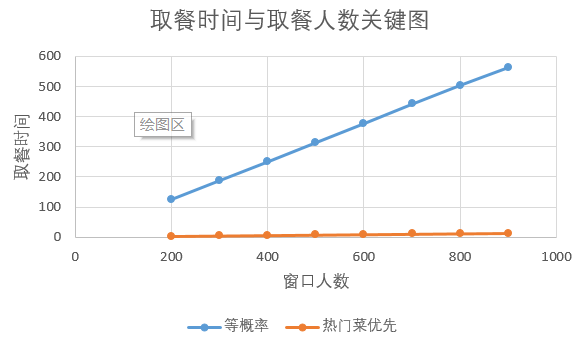
\includegraphics[scale=1]{./image/pic2.png}
  \caption{摆放方案效果图}
\end{figure}
\begin{center}
\begin{tabular}{|c|c|c|c|c|c|c|c|c|}
\hline
$N$&200&300&400&500&600&700&800&900\\
\hline
$t_1$&126.468&189.191&251.246&314.934&378.141&442.625&505.126&564.231\\
\hline
$t_2$&3.059&4.598&6.111&7.638&9.122&10.607&12.139&13.636\\
\hline
\end{tabular}\\
\end{center}


在以上三种模型问题的构建过程中。针对每种模型各自的研究优点以及缺陷,结合实际问题,选择合适的建模方法,对于解决实际问题具有重要意义。
\subsection{参考文献}
谁参考了来糊一个呗。
\section{附加部分}
\subsection{程序代码}
关于食堂的菜品摆放顺序问题,我们对于等概率摆放情况,以及优先摆放热门菜品的策略进行模拟,模拟所用代码如下:
\lstset{language=C++}
\lstset{
    numbers=left, 
    numberstyle= \tiny, 
    numberstyle= \color{red!30!green!90},
    keywordstyle= \color{ blue!70},
    commentstyle= \color{red!50!green!50!blue!50}, 
    frame=shadowbox, % 阴影效果
    rulesepcolor= \color{ red!20!green!20!blue!20} ,
    escapeinside=``, % 英文分号中可写入中文
    xleftmargin=2em,xrightmargin=2em, aboveskip=1em,
    framexleftmargin=2em
}
\begin{lstlisting}
#include <iostream>
#include <queue>
#include <ctime>
#include <cstdlib>
using namespace std;

#define maxp 40000

class Customer {
public:
	double wt;//wait time
	int prefer;//prefer which dish
	bool picked;//if he has picked his dish
	Customer(){}
	Customer(int n):wt(0),picked(false){
		prefer = genPrefer(n);
	}
	int genPrefer(int n) {
		//[1]equal probability
		//return rand() % n;

		//[2]inequal probability - linear - popular first
		int base = 0;
		for (int i = 1; i <= n; i++) base += i;
		int seed = rand() % base;
		int sum = 0;
		for (int i = 1; i <= n; i++) {
			if (seed >= sum && seed < sum + i) {
				return 30 - i;
			}
			sum += i;
		}
	}
};

int main() {
	//freopen("data.in", "r", stdin);
	int nw = 30;//number of windows
	int np = 40000;//number of total people
	int l; //length of a line
	int cnt;//number of people out
	double pick = 1.0f;//time for picking up dish
	Customer cq[maxp];//queue of customers
	//intialize
	srand(unsigned(time(NULL)));
	for (int i = 0; i < np; i++) {
		cq[i] = Customer(nw);
	}
	for (l = 20; l <= 90; l += 10) {
		cnt = 0;
		for (int i = 0; i < np; i++) {
			cq[i].picked = false;
			cq[i].wt = 0;
		}
		//start service
		int front = 0, tail = 0;//[front,tail] is the people in line
		//int kk = 0;
		while (cnt < np) {
			//cout << cnt << endl;
			//calculate blocking time
			//if (tail == np - 1) {
			//	cout << kk++ << endl;
			//}
			bool flag = false;
			for (int i = front; i <= tail; i++) {
				//perfer dish's window area:[prefer/nw,(prefer+1)/nw]
				//the position of customer:(tail-i)/l
				if (cq[i].picked == false) {
					double pwl = double(cq[i].prefer) / nw;
					double pwr = double(cq[i].prefer + 1) / nw;
					double pc = double(tail - i) / l;
					if (tail == np - 1) {
						//front -> l-1, front+1 -> l-2
						pc = double(l - i - 1 + front) / l;
					}
					//pick his favourite dish
					if (pc >= pwl && pc <= pwr) {
						cq[i].picked = true;
						//only one-time block
						if (flag == false) {
							for (int i = front; i <= tail; i++) {
								cq[i].wt += pick;
							}
							flag = true;
						}
					}
				}
			}
			//unfull
			if (tail == np - 1) {//out
				front++;
				cnt++;
			}
			else if (tail - front + 1 < l) {
				tail++;//in
			}
			//full
			else {
				front++;
				tail++;
				cnt++;
			}
		}
		double E = 0;
		for (int i = 0; i < np; i++) {
			E += cq[i].wt;
			//cout << cq[i].wt << endl;
		}
		E /= np;
		cout << "l:" << l << "\t" << "E:" << E << endl;
	}
	return 0;
}
\end{lstlisting} 

\subsection{课程感悟}
\paragraph{冯相}

\paragraph{王艺瑾}
我们小组在这篇课程论文上的进展并非一帆风顺。从最初的选题就经历了许多想法的碰撞和意见的磨合。虽然有许多主题最后被我们淘汰,但在一次次讨论的过程中,我们也发现了这些问题的各种拓展的可能性和研究方向,在之后有合适的机会时,它们仍然都是很值得研究的课题,如TSP问题,最小生成树问题等等。而在定完选题之后,我们小组又经过了许多轮讨论。最初的几次讨论我们一直关注着周期模型,在许多细节上也产生了较大的分歧,几次讨论之后仍然不能得到统一的意见。但最后经过老师的点拨,我们想到了更简洁但也贴近实际情况的概率模型,大大增加了模型的可行性。然而,即便我们在最后才想出完整的模型,之前的几次讨论仍然使我们的思维能力得到了训练,这些都是我们在这门课中得到的十分宝贵的经历。
\paragraph{徐润森}
我们最开始想到这个问题的时候认为,这一问题中人员的取餐行为非常明确,因此将会有唯一的答案。但是在实际建模中,假设的不同以及思考问题的切入点不同,会产生不同的评价指标,进而会建立起不同的数学模型。在建模过程中,我最大的收获还是与组员们互相讨论,碰撞思想的过程。我们的模型写出来之前,每个人都提出了无数的想法,这些想法一开始并不明确,但是这些不同的想法会给其他人带来灵感,提出更加完善可行的方法。比如说,在考虑周期模型的时候,我们从提出“阻塞由队列中位置最靠前的取菜的人引起”这一基本事实出发,推导出公式,进而慢慢搭建起整个模型,这一过程中,我们还反复思考发生阻塞的人在取菜走廊的相对位置是否会产生影响,最后得出不影响的结论,这是由周期的性质决定的。又比如我们在构建概率模型的过程中,转换角度从个体出发,结合期望相加的性质进而得出简洁的表达式并且进行推广,就经历了从复杂的思维中跳脱出来回归问题本质的过程,当然,这一过程还需要感谢老师的指点。总的来说,这次建模过程让我体会到了数学建模精益求精、永无止境的过程,更让我体会到了和靠谱队友分工协作的乐趣,收获了友谊。谢谢老师!
\paragraph{占子越}
数学建模的过程本身就是一个有趣的讨论过程,一个好模型的构建需要与实际问题有着紧密的联系,同时也要有着易于解决的途径。就排队问题而言,阻塞是对问题关键的很好的概括:排队与不排队的区别关键在于是否会发生阻塞,这是对问题的抽象。考虑阻塞时间,以及推倒出与总时间的关系,是对问题的解决。考虑每个位置上的阻塞期望和,其成功的关键在于既考虑到了位置的影响,又将每个人当前是否取菜的状态忽略,而转为考虑是发生阻塞时每个人否可能取菜,并将总时间期望由单次时间期望线性相加,简洁明了。
\paragraph{宗威旭}
在本次选题过程中,我们最后选择的建模过程相对是更具有挑战性的。对于食堂排队问题,我曾想过用组合优化或者处理逆序的过程实现。不过这些思路最后并没有成为成型的想法。在听队友们一起交流分享时,感觉自己产生了很多思路与想法,在选取较为容易研究的单次阻塞时间,并将每个人的取餐时间建立合理的映射,这是简化模型,成功分析的一个优秀的思路。中间过程中严格的公式推导,与利用程序设计对于实际问题的检验,又对我们的分析起到了支持作用。感觉在这一过程中的思考与收获时很大的。

\end{document}
